\chapter{扰动场作用下的热负荷分析}


% 在之前的研究中,研究者曾经用 GENRAY 相关代码将场线进行推测。

上一章中我们基于抑制 ELM 的需要提出了扰动场之间互相耦合的优化方法,这一章中我们进一步探究优化后的扰动场是否能够一定程度上缓解\Hmode 面对的热负荷问题。限于时间原因,以螺旋电流丝对热负荷分布的影响作为例子,探究外加扰动场控制热负荷的可能,可以调节材料受热的手段以材料损害。


如果粒子在刮削层中运动时不考虑场的横向方向上的输运,即不考虑碰撞的情况,则难以模拟打到偏滤器上的热负荷分布,粒子流分布非常集中。若是基于蒙特卡洛的思想,在粒子沿磁力线移动时引入横向漂移则可改善这一点。即粒子沿磁力线运动,但是每过一段满足指数分布的随机步长便发生横向漂移,使得粒子在不同磁力线之间可能发生漂移,在磁力线追踪程序的基础上添加了不确定性。
% 通过在一个边界磁面附近以均匀分布的种子为起点,计算打到偏滤器上各种负荷分布的计算。

\section{磁力线追踪与扩散}

  
磁力线追踪(\textit{F}ield \textit{L}ine \textit{T}racing, 磁力线追踪)是在磁场网格中进行插值和常微分方程求解得到真实磁场的磁力线分布的模拟手段。
磁力线追踪准备了插值和 ODE 的程序工具(Runge-Kutta 5 阶),可以产生迹线了(2D+3D),并且切换其他 ODE 数值计算方法相当方便。原有的 ERGOS 磁力线追踪似乎只能在磁面坐标系内进行 磁力线追踪,依据柱坐标进行重写之后可以在闭合磁面外追踪。


$$\dot{\vect{X}}(t) = \vect{B}(\vect{X}) $$

注意改变向量场的大小并不会改变上述常微分方程的轨迹,所以也可以有 $\dot{\vect{X}}(t) = \vect{B}/|\vect{B}| $,它仅改变到达轨迹上某点需要的时间。本论文中采用了 scipy 科学计算库中 integreate.ode 函数提供的龙格-库塔五阶方法,感兴趣的读者还可以在其提供的其他方法中进行选取。


当我们考虑粒子间的碰撞效应,粒子沿磁力线走过随机长度 $x$ 后发生一次横向漂移,

\begin{equation}
    p(x)=\frac{1}{\lambda} \exp \left(\frac{-x}{\lambda}\right),
\end{equation}

其中 $\lambda$ 为电子平均自由程。
横向漂移的方向在垂直于场的平面内随机均匀分布,而步长则在下面区间均匀随机分布,
\begin{equation}
  r \in[0, \sqrt{\frac{12 D_{\perp} \lambda}{v}}]
\end{equation}
其中 $D_{\perp}$ 为唯象的横向扩散系数而 $v$ 是电子速度。通过这种手段加入粒子扩散的因素可以一定程度上估计真实的热负荷分布。




% 尽管前一章节中对边界局域模的抑制是主要的评判扰动场的函数,评估热分布 $h(x,y)$ 优劣的函数,暂时选用梯度绝对值的 $\mathrm{L}^1$ 范数作为品质因子的计量标准,作为给定扰动场对应的热负荷分布的。
% \begin{equation}
%     \operatorname{FoM} =  \iint |\nabla h(x,y)| \mathrm{d} x \mathrm{d} y
% \end{equation}

\begin{figure}[htbp]
    \centering
    % \subcaptionbox{基于蒙特卡洛的磁力线扩散算法产生锯齿状的磁力线}{%
    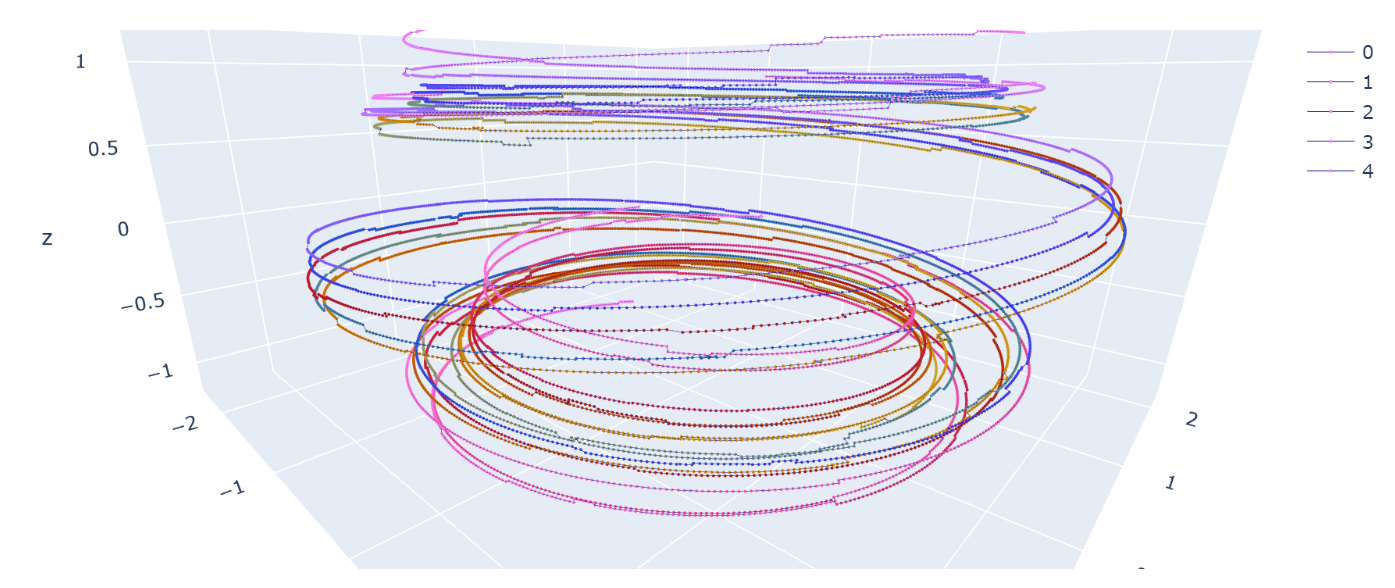
\includegraphics[width=0.80\columnwidth,keepaspectratio]{sawtooth_FLD.png}
    % }%
    \caption{基于蒙特卡洛的磁力线扩散算法产生锯齿状的磁力线}
\end{figure}


% The direction of the steps is uniform in the plane perpendicular to the field, while the step size $r$ is uniform in the interval:


该方法已在 Wendelstein 7-X 上成功应用以预估热负荷分布。

\section{螺旋电流丝作用下的热负荷分布}
我们在这一章中主要是通过磁力线的追踪和扩散技术来观察等离子体边界的磁拓扑变化,先从上偏滤器靶板附近邻域(由于该模拟位型是上单零位型)出发,射出磁力线,测量各磁力线长度和最深渗透 $s$,通过磁力线的长度我们可以判断其磁力线延伸后的簇状结构,即有哪些磁力线在追踪过程中仍是靠近的;通过最深渗透 $s$ 磁坐标半径可以判断能够射入等离子体最外闭合磁面内部的磁力线簇。如果热流和粒子流从等离子体中泵出的话,它们最有可能沿着能够深入等离子体的磁力线到其打击点上。

\subsection{原打击点附近的磁力线追踪模拟}
设置螺旋电流丝总电流大小设为 1.3 kAt,它引起了三维不对称的磁扰动结构,以 $n=1$ 主导,我们以它作为例子研究其引起的热负荷的分布的改变。
  
先在上偏滤器的一个邻域(环向联通)为起点进行磁力线追踪,对磁力线的延伸长度和最深渗透等离子体的 s,即径向半径进行直方图统计。

\begin{figure}[htbp]
  \centering
  
  \begin{subfigure}{0.4\textwidth}
    \includegraphics[width=0.9\columnwidth, keepaspectratio]{HCFs_EAST_73999/SP.png}
    \caption{磁力线追踪的起点,前后两个端点在极向切面上的分布,部分 磁力线追踪的计算到了时间限制停在了等离子体内。}
  \end{subfigure}%
  \begin{subfigure}{0.57\textwidth}
    \includegraphics[width=1.0\columnwidth, keepaspectratio]{HCFs_EAST_73999/hist.png}
    \caption{磁力线追踪的长度和最深渗透 $s$ 分布的直方图}
  \end{subfigure}%
  \caption{上沿偏滤器靶板邻域作磁力线追踪的起点的模拟统计结果}
\end{figure}



可以观察到在螺旋电流丝的影响下,能够深入等离子体内部的磁力线追踪在图上出现了打击点分裂的特征,即原有的打击点处于偏滤器固定位置,通过螺旋电流丝引起了偏滤器靶板上打击点的带状分裂。$n=1$ 主导的螺旋电流丝扰动场影响下,其磁力线的扰动也有 $n=1$ 的特征。

\begin{figure}[htbp]
  \centering%
      \includegraphics[width=1.0\columnwidth]{HCFs_EAST_73999/length_dist.png}
      \includegraphics[width=1.0\columnwidth]{HCFs_EAST_73999/min_s.png}
      \caption{上下两图分别显示偏滤器上出发的磁力线的特征参数,上图显示的是磁力线长度,下图显示的是最深渗透 $s$。y 轴表示的是从偏滤器低场侧中心开始算起到磁力线追踪起点的距离。}
\end{figure}

\subsection{等离子体边界附近的磁力线扩散模拟}
现在等离子体边界外围布满磁力线追踪的起点,并且设为具有随机性的磁力线扩散,对其进行统计分析和到偏滤器上的打击点分布分析。 

\begin{figure}[htbp]
    \centering
  \begin{subfigure}{0.4\textwidth}
    \includegraphics[width=0.9\columnwidth, keepaspectratio]{HCFs_EAST_73999_FLD/SP.png}
    \caption{磁力线追踪的起点,前后两个端点在极向切面上的分布,部分 磁力线追踪的计算到了时间限制停在了等离子体内。}
  \end{subfigure}%
  \begin{subfigure}{0.57\textwidth}
    \includegraphics[width=1.0\columnwidth, keepaspectratio]{HCFs_EAST_73999_FLD/hist.png}
    \caption{磁力线追踪的长度和最深渗透 $s$ 分布的直方图}
  \end{subfigure}%
  \caption{以等离子体边界作磁力线追踪的起点的模拟统计结果}
  \end{figure}
  
通过对磁力线在原打击点周围的分布进行计数测量,一定程度上证实了扰动场引起的打击点的分裂,图 \ref{fig:sp-on-divertor}, 但数据量较少。
  
\begin{figure}[htbp]
    \centering%
        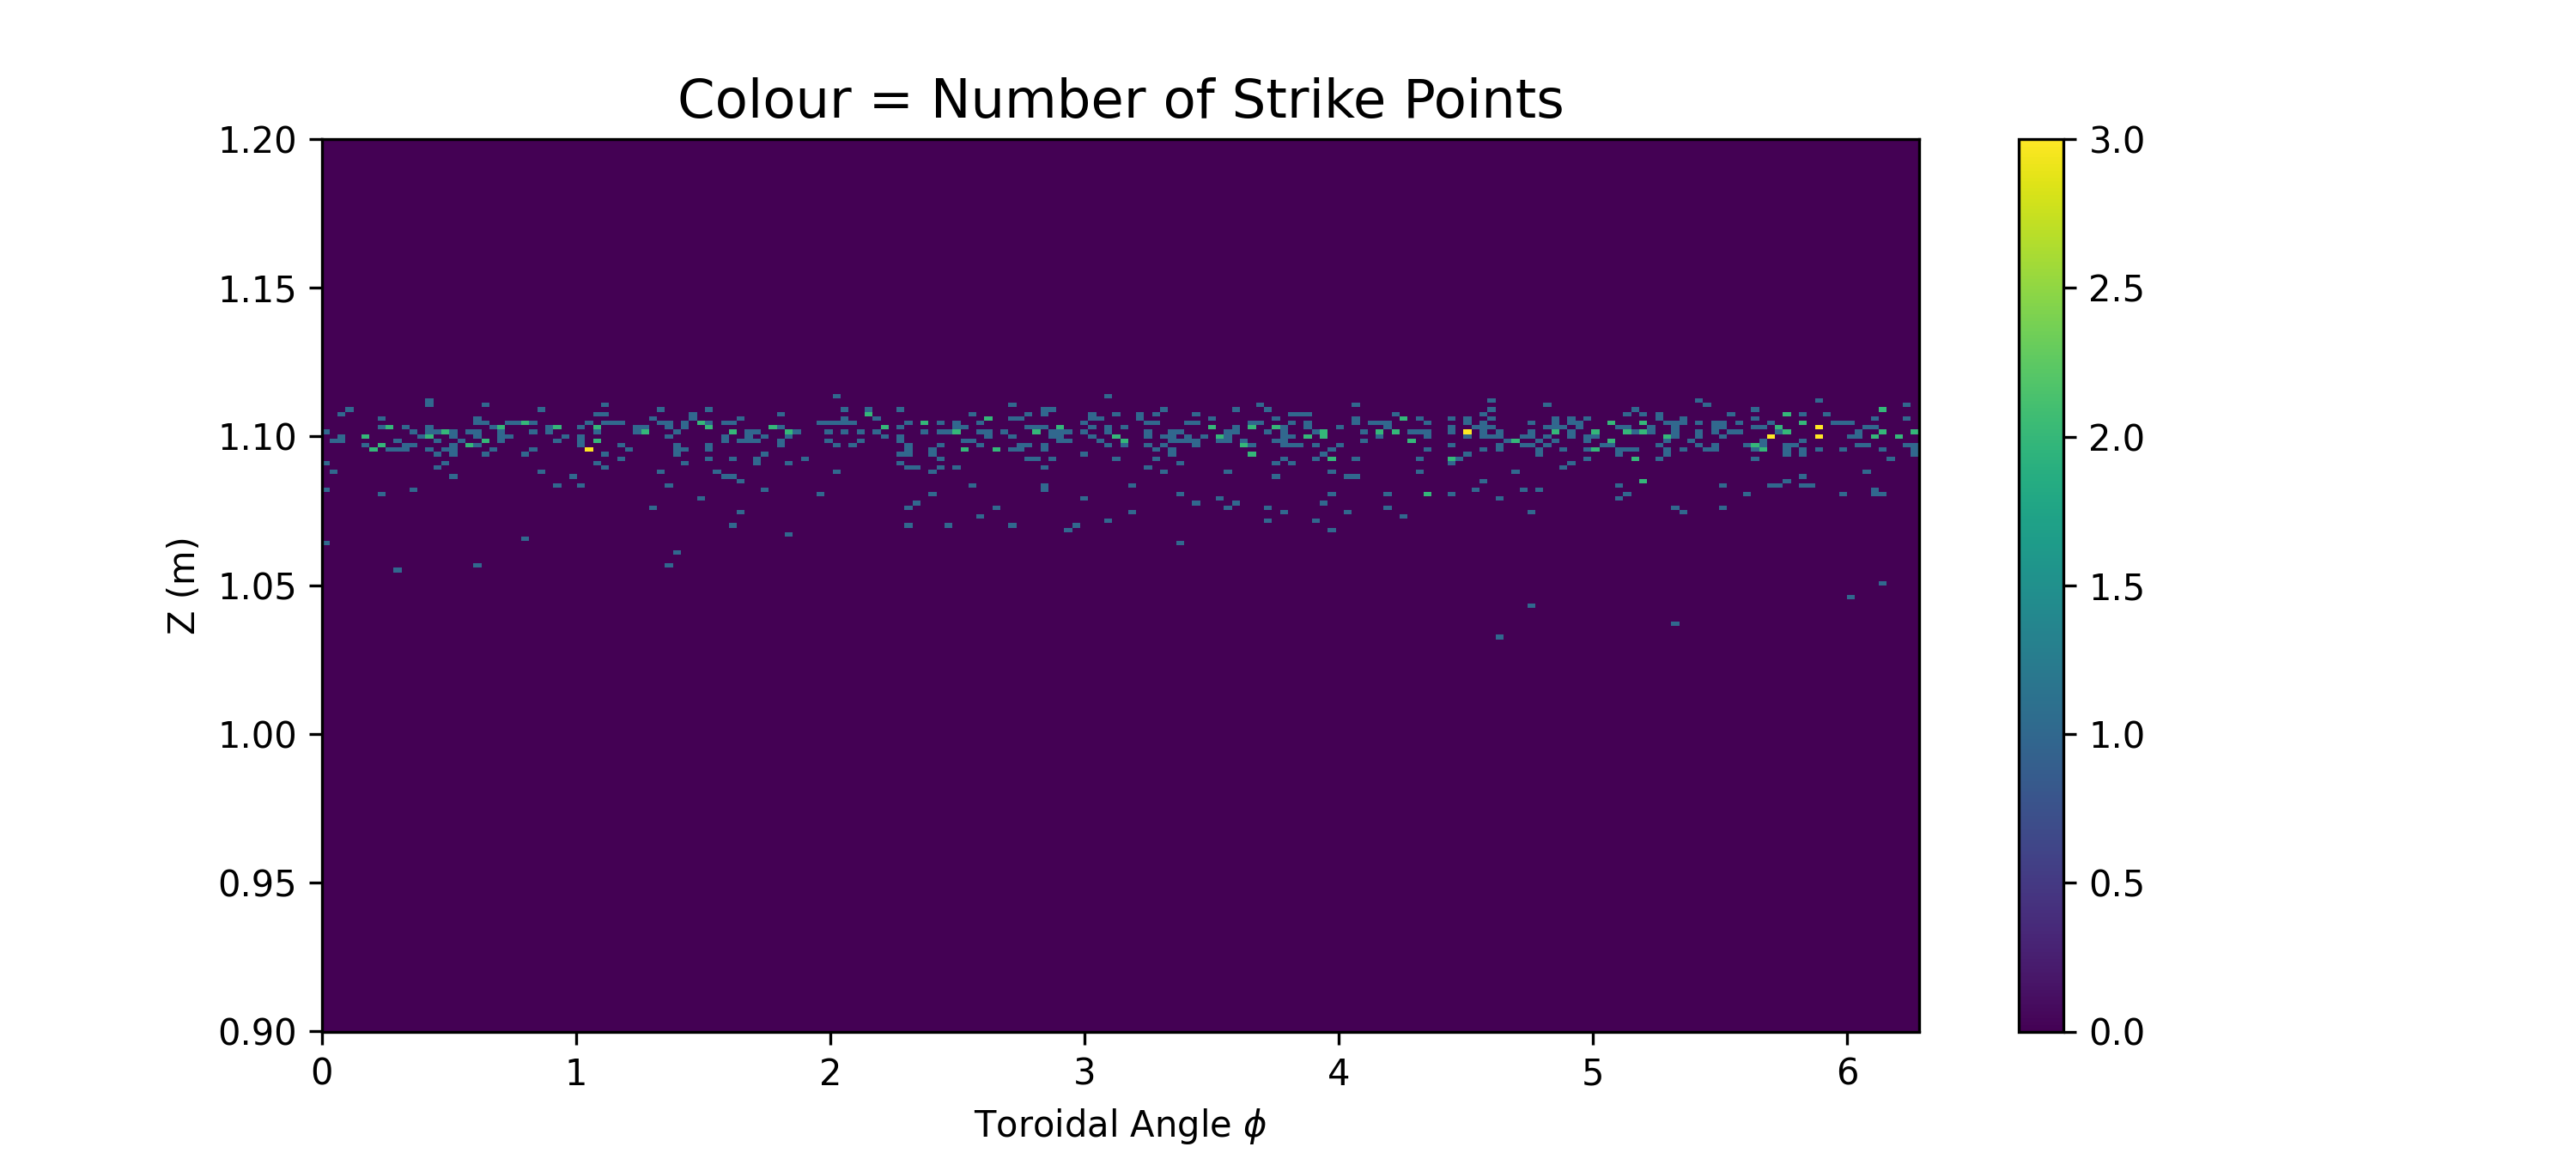
\includegraphics[width=0.70\columnwidth]{HCFs_EAST_73999_FLD/SP_dist.png}
        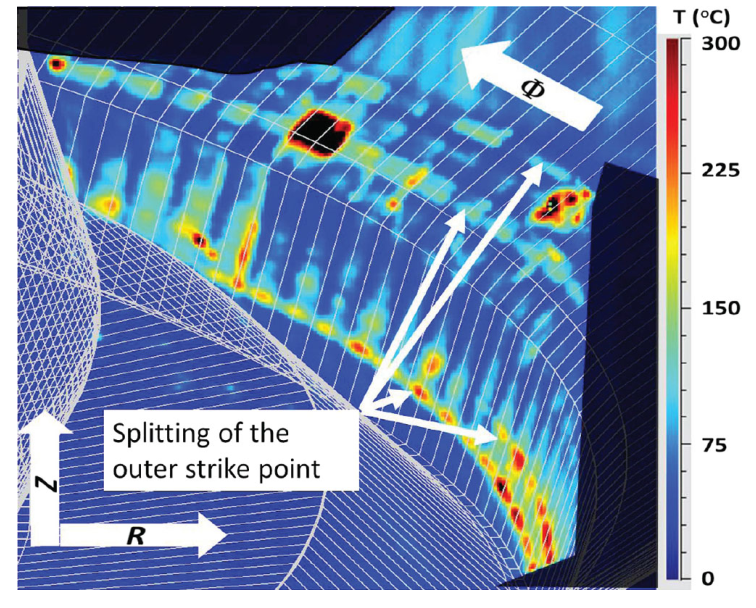
\includegraphics[width=0.29\columnwidth]{translate/liang_4.png}
        \caption{左图为等离子体边界上出发的磁力线扩散打到上偏滤器周围的能流密度(实际为二维直方图,计数为磁力线重点落在方格内的数目),右图为实际螺旋电流丝存在且为下单零位型时的下偏滤器旁温度分布,具体实验细节参见附录。}
        \label{fig:sp-on-divertor}
  \end{figure}

% 平衡场的磁力线追踪结果

% \begin{figure}[htbp]
%   \centering%
%       \includegraphics[width=1.0\columnwidth]{equili_EAST_73999/length_dist.png}
%       \includegraphics[width=1.0\columnwidth]{equili_EAST_73999/min_s.png}
%       \caption{平衡场的上偏滤器旁邻域内作起点进行 磁力线追踪,其最深渗透深度和长度分布。}
% \end{figure}


\section{小结}

本节通过基于蒙特卡洛思想的磁力线扩散模拟了可能的热负荷在偏滤器平板上的分布,未来该模拟结果可以与实验进行对比,验证热负荷估计的准确性。另一方面,这一结果初步揭示了通过非对称的扰动场,可以调节边界磁拓扑以调整粒子流及热负荷在偏滤器上的分布。

但仅仅如此还是不够的,如何对扰动场作用下偏滤器靶板上的磁力线落点位置进行归类总结,分析其形成的空间三维磁力线簇状结构是一个可以展开研究的重点内容。对这种有组织的三维结构的流场还需要细致的分析,不能单纯满足于算例的数值实验。